\title{Lab 1: Arduinos \& LEDs}
\author{Engineering 100-950}
\date{Winter 2022}
\documentclass[12pt]{article}
\usepackage[margin=1in]{geometry}
\usepackage{graphicx}
\usepackage{circuitikz}
\usepackage{fancyhdr}
\usepackage{hyperref}
\chead{Written \& Edited by Arun Nagpal, Sarah Redman, Scott Smith, Kitty Ascrizzi,\\
Grace Ochs, Camber Hortop, Jessica Fisher, Aaron Ridley}
\usepackage{hyperref}

\begin{document}
	\maketitle
	\thispagestyle{fancy}
	
	\section*{Materials}
	\begin{itemize}
		\item 1 \quad Arduino Nano 33 BLE
		\item 9 \quad LEDs
		\item 3 \quad 1-k$\Omega$ Resistors
		\item 3 \quad 2-k$\Omega$ Resistors
		\item 3 \quad 7.5-k$\Omega$ Resistors
		\item 3 \quad 10-k$\Omega$ Resistors
	\end{itemize}
	
	\section*{YouTube Video}
	\href{https://www.youtube.com/playlist?list=PLp2z0IQxLSvkKL0vEaFtbyeb6julsa3-8}{Feel free to watch the YouTube playlist at this link (Click Here). It should help you better understand LED circuits and basic Arduino programming.}
	
	\section*{Introduction}
    Welcome to ENGR100-950! Over the course of the next semester, you will be designing and building your own circuit board, complete with measurement instruments to gather information on all sorts of atmospheric data. To get to that point, we will spend the first couple labs learning about various components and eventually how to combine them into a cohesive system.\\
    
	In lecture, you've had a crash course on the ins and outs of microcontrollers. Now, you'll be working with your own \textbf{Arduino Nano 33 BLE} microcontroller so you can begin to learn how to use it. The Nano will be the brain of your payload; it is very well-suited to these sorts of applications, as you will see.\\
	
	The \textbf{input/output (IO) pins} on the Nano each serve different purposes. On the next page, there's a helpful diagram that details the types of pins on the board.\\
	
	\begin{figure}[h]
		\begin{center}
			\includegraphics[scale=0.5]{Figures/nano33ble-pinout.png}
			\caption{Photo Credit: forum.arduino.cc}
		\end{center}
	\end{figure}

	In general, the digital pins are on one side (D2-13), and the analog pins are on the other (A0 - A7). Digital pins only read and write binary values - HIGH (5V) or LOW (0V). Analog pins can also write these binary values. However, analog pins can read more than just binary values. They read a range of analog values from 0V - 5V. An analog pin reads the voltage that it `sees' on the circuit or sensor you connect it to. \\

	Finally, it's worth noting the GND pin. Voltage values are read with respect to some constant reference. They are \textbf{relative}, not \textbf{absolute}. This reference is usually called 'Ground.' There should ALWAYS be a ground connection on every circuit you make, whether you are using a microcontroller or not. This is essential when dealing with electricity, to make sure that things don't spark or get fried because they draw too much power.\\

	To illustrate, consider the simple LED circuit shown in Figure 2, where a 5V supply powers a bulb, which is attached to GND. The two circuits shown in Figure 2 are actually equivalent representations of the same thing. In the circuit on the left, the 5-volt battery raises the top half of the loop 5 volts higher than the bottom half. The bottom half of the loop is held at zero volts, since it is grounded. Current flows clockwise from the positive (top) to the negative (bottom) terminals of the battery.\\
    
    	\begin{figure}[h]
		\begin{center}
			\begin{circuitikz} \draw
				% First circuit
				(0, 0)	to [battery1, label={5V Batt.}]	(0,4) 
				(0, 4)	-- (4, 4)
				(4, 4)	to [full led, *-*]	
				(4, 0) -- (0, 0)
				(2, 0)	node[ground, label={[label distance=0.8cm]below:GND}]{}
				% Second circuit
				(7, 0)	node[ground, label={[label distance=0.8cm]below:GND}]{}
				(7, 4)	to [full led, o-*]	(7, 0)
				(7, 4)	node[label={above:5V}]{}
				;
			\end{circuitikz}
		\end{center}
		\caption{A simple circuit powering an LED}
	\end{figure}
	
	In the circuit on the right, the top node is held at 5V by some unseen source, and the bottom is held at 0V because it is grounded. The current flows down, into the grounded node. This representation works great if you want to analyze a fragment from a larger circuit.
	
	\section{The Breadboard}
	
	Before actually launching into the building of circuits, it's important to understand the tools that you are working with. Your breadboard will act as the `circuit board' on which you build your systems. Notice that it is organized by enumerated rows and columns. \\
	
	The pins of the electronic devices go into the holes in the breadboard. These holes are related to each other in that every row of 5, as defined on the board, are electrically connected. This means that if, for instance, you connect a 5V battery to a given hole, all of the holes in that row are raised to 5V. \\
	
	Circuit elements are connected in breadboards by connecting the input pins of one device to the same row as the output pins of another device. In this way, devices can be chained together to create complex circuits. An example is shown below (Fig. 3). This circuit is called a voltage divider, and consists of two resistors connected end to end. A formal circuit diagram of a voltage divider is shown later in this manual (Fig. 5). \\
	
	\begin{figure}
		\begin{center}
			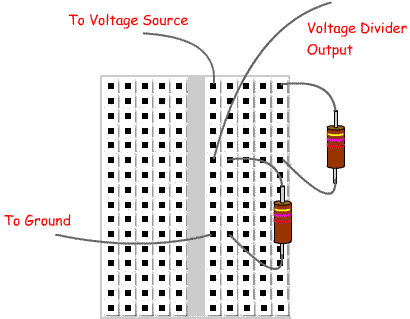
\includegraphics[width=\linewidth]{Figures/voltagedivider.png}
			\caption{Photo Credit: electroschematics.com}
		\end{center}
		\begin{center}
			\begin{circuitikz} \draw
				(0, 4)	node[label={above:$V_{in}$}]{}
				(0, 4)	to [R, o-*, label={2-k$\Omega$}]	(0, 2)
				(0, 2)	to [full led, *-*]	(0, 0)
				(0, 0)	node[ground, label={[label distance=0.8cm]below:GND}]{}
				;
			\end{circuitikz}
		\end{center}
		\caption{LED circuit to be built, use the Arduino 5V pin for $V_{in}$}
	\end{figure}
	
	Your lab instructors will demonstrate using a breadboard before the lab begins. If you have questions about whether or not you are connecting devices appropriately, please don`t hesitate to ask.
	
	\begin{enumerate}
		
		\item Ensure that either your computer or your partner's computer has a USB-A port.
		
		\item Build the LED circuit shown in Fig. 4. When built, it should look similar to the voltage divider circuit in Fig. 3, except one of the resistors will now be an LED. Be aware that LEDs only turn on when placed in your circuit in the correct orientation. Try switching the orientation of your LED if it doesn't turn on after completing step 2.
		(hint: one leg is longer than the other!)
		
		\item Turn on the Arduino by plugging in the micro USB cord into the device and the USB into the computer. Note that an LED built into the microcontroller should begin glowing. The LED you connected to the Arduino should also begin to glow if your circuit is correct.
	\end{enumerate}
	
	\section{LED Blink}
	\begin{enumerate}
		
		\item Let’s run some example scripts. Open up the Arduino Integrated Development Environment (IDE) on your computer or through CAEN Virtual Sites and go to File $\rightarrow$ Examples $\rightarrow$ Basics $\rightarrow$ Blink. A new window should open up, with some code on it. (Make sure to set the proper microcontroller and processor under the Tools menu). Upload and run the code, and observe what happens.
	
		\item Change your code so that the LED that turns on and off is the external one, not the built-in one. You'll need to connect your LED to a digital pin instead of the 5V pin. Don't forget to initialize the digital pin in setup(). Test it and make sure it works. 
		
		{\raggedright{}Save your code and rename it to something more recognizable. It will be prudent to create a new folder on the computer to store these scripts for easy recollection later. You will be submitting this program, so make sure to keep it.}
	
		\item Copy your code to a new page, and alter it so that the LED is on for 2 seconds and off for half a second, but after every 5 cycles of this, it 'rests' by turning off for 5 seconds. Do this in only 2 additional lines. Keep this code, as it is the second file you will be submitting later.
	
		\item Connect 8 more LEDs to the Arduino digital out pins and ground them with one resistor. Write a new Arduino script to approximate the behavior of the light in the beginning of the video below (so that the light shifts left and right at a constant speed). Try to write this program with less than 20 lines in loop. If you're a "Knight Rider" fan, come tell your instructors for brownie points. Make sure to save this code, as you will be submitting it. You should have three separate programs saved so far. \\ (\url{https://www.youtube.com/watch?v=FpyKlLuLbcs})
	\end{enumerate}
	
	\section{Voltage Divider}
	Consider a \textbf{voltage divider} shown below. The output voltage is related to the input voltage through the equation
	$$ V_{out} = \frac{R_{2}}{R_1 + R_2} V_{in} $$
	\begin{figure}[h]
		\begin{center}
			\begin{circuitikz} \draw
				(0, 4)	node[label={above:$V_{in}$}]{}
				(0, 4)	to [R, o-*, label={$R_1$}]	(0, 2)
				(0, 2)	to [short, -o]				(2, 2)
				(2, 2)	node[label={above:$V_{out}$}]{}
				(0, 2)	to [R, *-*, label={$R_2$}]	(0, 0)
				(0, 0)	node[ground, label={[label distance=0.8cm]below:GND}]{}
				;
			\end{circuitikz}
		\end{center}
		\caption{A generic voltage divider}
	\end{figure}
	Note the order of the resistors - getting them confused will lead you to the wrong value. The concept of the voltage divider can be extended to any number of resistors. The output voltage at each node is simply the total resistance below that node divided by the total resistance of the circuit. As you might have guessed from the formula, when resistances are placed \textbf{in-series} like so, their resistances add. Make sure you understand the concept, you'll need it for future labs.

	\begin{enumerate}
        \item Disassemble any circuits you have from the previous parts of the lab. Plug a wire directly from the 5V line of the Arduino into A2 of the Arduino. Create a new Arduino program and use the analogRead() function to read in the voltage. Look up how Serial works for Arduino to write this program. The specifics can be found online, but first you need to initiate communications between the Arduino and your computer using Serial.begin(9600). The 9600 specifies the baud rate, and lets the Arduino know how fast to send data to the computer. Serial.print(dataHere) prints dataHere. The variable dataHere can be data of many types, including integers, doubles, and character arrays. To see the data sent from the Arduino to the computer, open the Serial monitor inside of the Arduino IDE. This can be done by clicking the magnifying glass in the top, left-hand corner of the IDE. At the bottom of the Serial monitor, make sure the baud rate is set at 9600 to match the Arduino. Record the value returned by analogRead(), as you'll need it later.
        
    	\item Build a voltage divider by setting $V_{in}$ as the 5V line of the Arduino, have $R_1$ be 2$k\Omega$ and $R_2$ be 2$k\Omega$. Plug $V_{out}$ into A1 of the Arduino.  Use the analogRead() function to read in the voltage and record the raw number that the function returns.
    
        Try playing with various resistor values, and take down the values from two more combinations of resistors. Make sure to write down the resistor combinations as well as the analog output for both of your additional experiments.
        
		\item Come up with a combination of resistors that will result in an output voltage of less than 1.25V. You can convert the raw output from analogRead() into voltage values by multiplying by 5/1024. You will learn why in next week's lab! Try it and see if it works. Now answer post lab question 1. Save this code, as it will be the fourth script that you submit.
		
        \item Write a script that turns on the LED if the voltage seen on A1 is 1.25V, but leaves it off otherwise. Test it with various combinations of resistors. You may have to add some ''wiggle room,'' (error margin), in your code around 5 mV. In addition, you may have to use more than 2 resistors. Remember that the resistance of resistors in series add. Save this code, as you will be submitting it. This should be your fifth and final coding file that you will submit. Now answer post lab question 2.
	\end{enumerate}

	\section*{Post Lab Questions}
	For this lab, you and your partner may discuss the questions but must submit unique answers to the post lab questions. 
	
	\begin{enumerate}
	    \item What combination of resistors did you use to get to less than 1.25V at the analog pin in step 3.3? Draw them in a circuit so it's clear where you put the resistors. You can draw it however you'd like as long as it is clear. What value will analogRead() return if it were to be used to measure a voltage of 1.25V?
	    
	    \item Draw the circuit you used to get to a value of approximately 1.25V in step 3.4. Make sure to label the values of the resistors you used in the diagram.
	    
	    \item What is a major difference between the digital and analog pins on the Arduino Nano?
	    
	    \item State the importance of having a ground (GND) in any circuit.
	    
		\item What does the pinMode() command do? Why is it necessary in the Blink.ino file? Read the documentation on the digital pins, and ask us questions if you have them. Use your favorite search engine to find the website!
		
		\item Describe your additions to the Blink.ino file in order for it to perform to the constraints defined in part 2.3.
		
		% \item Redraw the circuit diagram of the voltage divider from Figure 5 in the form of the leftmost 'looped' circuit like in Figure 2.
		
        \item Why are the voltage values returned the way they are by analogRead() (i.e. not standard voltage values)? Try reading about analogRead() on the Arduino forums. 
        
        % \item Plot, by hand or in MATLAB, the values returned by analogRead() and their corresponding calculated voltage by using the voltage divider equation for the data collected in 3.1, 3.2, and 3.3. Include the plot in your response. How are these data points related? It's likely there is some slight deviation from what you would expect. Why might there be this deviation (if you don't have any deviation, come up with reasons that could cause some)? Describe an equation that maps from analogRead() values directly to voltage and explain your reasoning.
        
		\item Using three resistors, draw a voltage divider circuit with two $V_{out}s$. $V_{out1}$ should be equal to 2/3 * $V_{in}$, and $V_{out2}$ should be equal to  1/3 * $V_{in}$. Draw the circuit in both styles as described by Figure 2. Give possible values those resistors could take. What would happen if we doubled the value of all of the resistors? 
		
		\item Can you build a voltage divider that produces an output that is higher than the input voltage? Why or why not?
		
		%\item A different microcontroller has an 8-bit analog to digital converter (ADC). It also measures values between 0 and 5V. If 5V is put into the ADC, what value would we see at the output?
		
	   	% \item Look up what baud rate means on the Arduino website. You can find this information under the info for Serial.begin(). What are the units? Convert a baud rate of 9600 into units of bytes/minute. 
	\end{enumerate}

    %\newpage
    
    \section*{Documentation}
    On Canvas, turn in the following files. Your answers to the post lab questions must be your own work, but the Arduino scripts may be the same as your partner's.
    \begin{enumerate}
        \item A PDF document that contains answers to the post lab questions.
        \item The modified LED Blink script (.ino) from 2.2.
        \item The further modified LED Blink script (.ino) from 2.3.
        \item The Knight Rider script (.ino) from 2.4.
        \item The script (.ino) used to test different resistor combinations for a voltage divider from 3.1-3.3.
        \item The script (.ino) to turn on the LED if the voltage on A1 was 1.25V from 3.4.
    \end{enumerate}
\end{document}

